\documentclass[12pt,utf8,notheorems,compress,t]{beamer}
\usepackage{etex}

\usepackage{pgfpages}
\setbeameroption{show notes on second screen}
\setbeamertemplate{note page}[plain]
\newcommand{\jnote}[2]{\only<#1>{\note{\setlength\parskip{\medskipamount}\justifying\footnotesize#2\par}}}
%\newcommand{\jnote}[2]{}

% Workaround for the issue described at
% https://tex.stackexchange.com/questions/164406/beamer-using-href-in-notes.
\newcommand{\fixedhref}[2]{\makebox[0pt][l]{\hspace*{\paperwidth}\href{#1}{#2}}\href{#1}{#2}}

\usepackage[english]{babel}

\usepackage{graphbox}
\usepackage{mathtools}
\usepackage{booktabs}
\usepackage{stmaryrd}
\usepackage{array}
\usepackage{ragged2e}
\usepackage{multicol}
\usepackage{tabto}
\usepackage{xstring}
\usepackage{ifthen}
\usepackage[normalem]{ulem}
\usepackage[all]{xy}
\xyoption{rotate}
\usepackage{tikz}
\usetikzlibrary{calc,shapes,shapes.callouts,shapes.arrows,patterns,fit,backgrounds,decorations.pathmorphing,positioning}
\hypersetup{colorlinks=true}

\usepackage{pifont}
\newcommand{\cmark}{\ding{51}}
\newcommand{\xmark}{\ding{55}}
\DeclareSymbolFont{extraup}{U}{zavm}{m}{n}
\DeclareMathSymbol{\varheart}{\mathalpha}{extraup}{86}

\graphicspath{{images/}}

\usepackage[protrusion=true,expansion=true]{microtype}

\setlength\parskip{\medskipamount}
\setlength\parindent{0pt}

\title{Generalized spaces for constructive algebra}
\author{Ingo Blechschmidt}
\date{September 2019}

\useinnertheme[shadow=true]{rounded}
\setbeamerfont{block title}{size={}}

\useinnertheme{rectangles}

\usecolortheme{orchid}
\usecolortheme{seahorse}
\definecolor{mypurple}{RGB}{150,0,255}
\setbeamercolor{structure}{fg=mypurple}
\definecolor{myred}{RGB}{150,0,0}
\setbeamercolor*{title}{bg=myred,fg=white}
\setbeamercolor*{titlelike}{bg=myred,fg=white}
\setbeamercolor{frame}{bg=black}

\usefonttheme{serif}
\usepackage[T1]{fontenc}
\usepackage{libertine}

% lifted from https://arxiv.org/abs/1506.08870
\DeclareFontFamily{U}{min}{}
\DeclareFontShape{U}{min}{m}{n}{<-> udmj30}{}
\newcommand\yon{\!\text{\usefont{U}{min}{m}{n}\symbol{'210}}\!}

\newcommand{\A}{\mathcal{A}}
\newcommand{\B}{\mathcal{B}}
\renewcommand{\C}{\mathcal{C}}
\newcommand{\M}{\mathcal{M}}
\renewcommand{\AA}{\mathbb{A}}
\newcommand{\E}{\mathcal{E}}
\newcommand{\F}{\mathcal{F}}
\renewcommand{\G}{\mathcal{G}}
\newcommand{\J}{\mathcal{J}}
\newcommand{\GG}{\mathbb{G}}
\renewcommand{\O}{\mathcal{O}}
\newcommand{\K}{\mathcal{K}}
\newcommand{\NN}{\mathbb{N}}
\newcommand{\QQ}{\mathbb{Q}}
\newcommand{\RR}{\mathbb{R}}
\newcommand{\TT}{\mathbb{T}}
\newcommand{\PP}{\mathbb{P}}
\newcommand{\ZZ}{\mathbb{Z}}
\newcommand{\CC}{\mathbb{C}}
\renewcommand{\P}{\mathcal{P}}
\newcommand{\aaa}{\mathfrak{a}}
\newcommand{\ppp}{\mathfrak{p}}
\newcommand{\fff}{\mathfrak{f}}
\newcommand{\defeq}{\vcentcolon=}
\newcommand{\defeqv}{\vcentcolon\equiv}
\newcommand{\Sh}{\mathrm{Sh}}
\newcommand{\GL}{\mathrm{GL}}
\newcommand{\Zar}{\mathrm{Zar}}
\newcommand{\op}{\mathrm{op}}
\newcommand{\Set}{\mathrm{Set}}
\newcommand{\Eff}{\mathrm{Ef{}f}}
\newcommand{\Sch}{\mathrm{Sch}}
\newcommand{\Aff}{\mathrm{Aff}}
\newcommand{\Ring}{\mathrm{Ring}}
\newcommand{\LocRing}{\mathrm{LocRing}}
\newcommand{\LRS}{\mathrm{LRS}}
\newcommand{\Hom}{\mathrm{Hom}}
\newcommand{\Spec}{\mathrm{Spec}}
\newcommand{\lra}{\longrightarrow}
\newcommand{\RelSpec}{\operatorname{Spec}}
\renewcommand{\_}{\mathpunct{.}}
\newcommand{\?}{\,{:}\,}
\newcommand{\speak}[1]{\ulcorner\text{\textnormal{#1}}\urcorner}
\newcommand{\ul}[1]{\underline{#1}}
\newcommand{\affl}{\ensuremath{{\ul{\ensuremath{\AA}}^1}}}
\newcommand{\Ll}{\text{iff}}
\newcommand{\inv}{inv.\@}
\newcommand{\seq}[1]{\mathrel{\vdash\!\!\!_{#1}}}
\newcommand{\hg}{\mathbin{:}}  % homogeneous coordinates
\newcommand{\brak}[1]{{\llbracket{#1}\rrbracket}}
\newcommand{\pt}{\mathrm{pt}}
\newcommand{\Loc}{\mathrm{Loc}}
\newcommand{\Top}{\mathrm{Top}}

\setbeamertemplate{blocks}[rounded][shadow=false]

\newenvironment{indentblock}{%
  \list{}{\leftmargin\leftmargin}%
  \item\relax
}{%
  \endlist
}

% Adapted from https://latex.org/forum/viewtopic.php?t=2251 (Stefan Kottwitz)
\newenvironment<>{hilblock}{
  \begin{center}
    \begin{minipage}{9.05cm}
      \setlength{\textwidth}{9.05cm}
      \begin{actionenv}#1
        \def\insertblocktitle{}
        \par
        \usebeamertemplate{block begin}}{
        \par
        \usebeamertemplate{block end}
      \end{actionenv}
    \end{minipage}
  \end{center}}

\newcommand{\bignumber}[1]{
  \renewcommand{\insertenumlabel}{#1}\scalebox{1.5}{\usebeamertemplate{enumerate item}}
}
\newcommand{\bigheart}{
\includegraphics{heart}}

\newenvironment{changemargin}[2]{%
  \begin{list}{}{%
    \setlength{\topsep}{0pt}%
    \setlength{\leftmargin}{#1}%
    \setlength{\rightmargin}{#2}%
    \setlength{\listparindent}{\parindent}%
    \setlength{\itemindent}{\parindent}%
    \setlength{\parsep}{\parskip}%
  }%
  \item[]}{\end{list}}

\tikzset{
  invisible/.style={opacity=0,text opacity=0},
  visible on/.style={alt={#1{}{invisible}}},
  alt/.code args={<#1>#2#3}{%
    \alt<#1>{\pgfkeysalso{#2}}{\pgfkeysalso{#3}}}
}

\newcommand{\pointthis}[3]{%
  \tikz[remember picture,baseline]{
    \node[anchor=base,inner sep=0,outer sep=0] (#2) {#2};
    \node[visible on=#1,overlay,rectangle callout,rounded corners,callout relative pointer={(0.3cm,0.5cm)},fill=blue!20] at ($(#2.north)+(-0.1cm,-1.1cm)$) {#3};
  }%
}

\tikzset{
  invisible/.style={opacity=0,text opacity=0},
  visible on/.style={alt={#1{}{invisible}}},
  alt/.code args={<#1>#2#3}{%
    \alt<#1>{\pgfkeysalso{#2}}{\pgfkeysalso{#3}}}
}

\newcommand{\hcancel}[5]{%
  \tikz[baseline=(tocancel.base)]{
    \node[inner sep=0pt,outer sep=0pt] (tocancel) {#1};
    \draw[red!80, line width=0.4mm] ($(tocancel.south west)+(#2,#3)$) -- ($(tocancel.north east)+(#4,#5)$);
  }%
}

\newcommand{\explain}[7]{%
  \tikz[remember picture,baseline]{
    \node[anchor=base,inner sep=2pt,outer sep=0,fill=#3,rounded corners] (label) {#1};
    \node[anchor=north,visible on=<#2>,overlay,rectangle callout,rounded corners,callout
    relative pointer={(0.0cm,0.5cm)+(0.0cm,#6)},fill=#3] at ($(label.south)+(0,-0.3cm)+(#4,#5)$) {#7};
  }%
}

\newcommand{\explainstub}[2]{%
  \tikz[remember picture,baseline]{
    \node[anchor=base,inner sep=2pt,outer sep=0,fill=#2,rounded corners] (label) {#1};
  }%
}

\newcommand{\squiggly}[1]{%
  \tikz[remember picture,baseline]{
    \node[anchor=base,inner sep=0,outer sep=0] (label) {#1};
    \draw[thick,color=red!80,decoration={snake,amplitude=0.5pt,segment
    length=3pt},decorate] ($(label.south west) + (0,-2pt)$) -- ($(label.south east) + (0,-2pt)$);
  }%
}

% Adapted from https://latex.org/forum/viewtopic.php?t=2251 (Stefan Kottwitz)
\newenvironment<>{varblock}[2]{\begin{varblockextra}{#1}{#2}{}}{\end{varblockextra}}
\newenvironment<>{varblockextra}[3]{
  \begin{center}
    \begin{minipage}{#1}
      \begin{actionenv}#4
        {\centering \hil{#2}\par}
	\def\insertblocktitle{}%\centering #2}
        \def\varblockextraend{#3}
	\usebeamertemplate{block begin}}{
        \par
        \usebeamertemplate{block end}
        \varblockextraend
      \end{actionenv}
    \end{minipage}
  \end{center}}

\setbeamertemplate{headline}{%
  \begin{beamercolorbox}[wd=\paperwidth,ht=2.25ex]{}%
    \insertsectionnavigationhorizontal{\paperwidth}{}{}%
  \end{beamercolorbox}%
  \vskip0pt%
}

\setbeamertemplate{frametitle}{%
  \vskip0.4em%
  \leavevmode%
  \begin{beamercolorbox}[dp=1ex,center]{}%
  %   \usebeamercolor[fg]{item}{\textbf{{\Large \insertframetitle}}}
    \begin{tikzpicture}
      \def\R{8pt}
      \node (title) {\hil{\large\,\!\insertframetitle}};
      \begin{pgfonlayer}{background}
        \draw[decorate, very thick, draw=mypurple]
          ($(title.south west) + (\R, 0)$) arc(270:180:\R) --
          ($(title.north west) + (0, -\R)$) arc(180:90:\R) --
          ($(title.north east) + (-\R, 0)$) arc(90:0:\R) --
          ($(title.south east) + (0, \R)$) arc(0:-90:\R) --
          cycle;
      \end{pgfonlayer}
    \end{tikzpicture}
  \end{beamercolorbox}%
  \vskip-0.6em%
}

\setbeamertemplate{navigation symbols}{}

\newcounter{framenumberpreappendix}
\newcommand{\backupstart}{
  \setcounter{framenumberpreappendix}{\value{framenumber}}
}
\newcommand{\backupend}{
  \addtocounter{framenumberpreappendix}{-\value{framenumber}}
  \addtocounter{framenumber}{\value{framenumberpreappendix}}
}

\newcommand{\insertframeextra}{}
\setbeamertemplate{footline}{%
  \begin{beamercolorbox}[wd=\paperwidth,ht=2.25ex,dp=1ex,right,rightskip=1mm,leftskip=1mm]{}%
    % \inserttitle
    \hfill
    \insertframenumber\insertframeextra\,/\,\inserttotalframenumber
  \end{beamercolorbox}%
  \vskip0pt%
}


\newcommand{\hil}[1]{{\usebeamercolor[fg]{item}{\textbf{#1}}}}
\newcommand{\bad}[1]{\textcolor{red!90}{\textnormal{#1}}}

\begin{document}

\addtocounter{framenumber}{-1}

\tikzstyle{topos} = [draw=mypurple, very thick, rectangle, rounded corners, inner sep=5pt, inner ysep=10pt]
\tikzstyle{title} = [fill=mypurple, text=white]

% Taken from Todd Lehman (CC-BY-SA) at https://tex.stackexchange.com/a/44920/32372

\newcommand{\setisprime}[1]{
  % Sets \isprime based on #1.
  \ifnum#1=1 \gdef\isprime{0} \else \gdef\isprime{1} \fi
  \foreach \sip in {2, 3,5,...,#1} {
    \pgfmathparse{\sip*\sip>#1? 1:0}
    \ifthenelse{\pgfmathresult=1}{
      % Early-out if \sip^2 > #1.
      \breakforeach
    }{
      % Otherwise test if \sip divides #1.
      \pgfmathparse{Mod(#1,\sip)==0? 1:0}
      \ifthenelse{\pgfmathresult=1}{
        \gdef\isprime{0}
        \breakforeach
      }{}
    }
  }
}

\newcommand{\setxy}[1]{
  % Sets \x and \y to loction of cell #1.
  \pgfmathtruncatemacro{\x}{Mod(#1-1,\cols)}
  \pgfmathtruncatemacro{\y}{(#1-1) / \cols}
  \pgfmathtruncatemacro{\y}{\cols - 1 - \y}
  \pgfmathparse{2.5*(\x+.5)}\let\x\pgfmathresult
  \pgfmathparse{2.5*(\y+.5)}\let\y\pgfmathresult
}

\newcommand{\numlabel}[2]{
  % Draws label #2 at cell #1.
  \setxy{\n}
  \node[fill=none, text=black] at (\x,\y) {#2};
}

\newcommand{\drawpolygon}[2]{
  % Draws polygon with #2 vertexes at cell #1.
  \setxy{#1}
  \ifthenelse{#2>1}{ % Polygon must have at least 2 sides.
    \ifthenelse{#2<30}{ % Draw polygon if it has a small number of sides.
      \filldraw (\x,\y) +(90:1)
      \foreach \drawi in {1,...,#2} {-- +(\drawi/#2*360+90:1)} -- cycle;
    }{ % Else approximate with circle.
      \filldraw (\x,\y) circle(1);
    }
  }{}
}

\newcommand{\setpolygoncolor}[1]{
  % Sets color based on #1.
  \gdef\polycolor{black}
  \ifnum#1=2\gdef\polycolor{black!50!white}\fi
  \ifnum#1=3\gdef\polycolor{yellow!95!red}\fi
  \ifnum#1=5\gdef\polycolor{yellow!0!red}\fi
  \ifnum#1=7\gdef\polycolor{blue!75!green}\fi
  \ifnum#1=11\gdef\polycolor{blue!70!red}\fi
  \ifnum#1=13\gdef\polycolor{blue!40!red}\fi
  \ifnum#1=17\gdef\polycolor{green!50!blue}\fi
  \ifnum#1=19\gdef\polycolor{green!80!black}\fi
  \ifnum#1=23\gdef\polycolor{green!50!red}\fi
  \ifnum#1=29\gdef\polycolor{yellow!50!black}\fi
  \ifnum#1=31\gdef\polycolor{orange!50!black}\fi
  \ifnum#1=37\gdef\polycolor{red!50!black}\fi
  \ifnum#1=41\gdef\polycolor{purple!50!black}\fi
  \ifnum#1=43\gdef\polycolor{blue!50!black}\fi
  \ifnum#1=47\gdef\polycolor{green!50!black}\fi
  \ifnum#1=53\gdef\polycolor{white!50!black}\fi
  \ifnum#1=59\gdef\polycolor{white!50!black}\fi
  \ifnum#1=61\gdef\polycolor{white!50!black}\fi
  \ifnum#1=67\gdef\polycolor{white!50!black}\fi
}

\newcommand{\sieve}[2]{
  \def\cols{#1}
  \def\rows{#2}
  \begin{tikzpicture}[scale=.5]
  \pgfmathtruncatemacro{\nmax}{\rows * \cols}

  \foreach \n in {1,...,\nmax} {
    \begin{scope}[fill=gray, fill opacity=.05,
                  draw=gray, draw opacity=.10,
                  line width=4]
      \drawpolygon{\n}{\n}
    \end{scope}
    \setisprime{\n}
    \ifthenelse{\isprime=1}{
      \numlabel{\n}{\bf\n}
    }{
      \def\startintensity{.33}
      \def\incrintensity{.10}
      \def\intensity{\startintensity}

      \def\m{\n}
      \pgfmathtruncatemacro{\i}{\m / 2}

      % Divide \m by \i until \m is extinguished.
      % Increment \i each time it does not divide into \m.
      \whiledo{\m>1}{
        \setisprime{\i}
        \pgfmathparse{Mod(\m,\i)==0? 1:0}
        \ifthenelse{\pgfmathresult=1\and\isprime=1}{
          \setpolygoncolor{\i}
          \begin{scope}[fill=\polycolor, fill opacity=\intensity,
                        draw=\polycolor!85!black, draw opacity=\intensity,
                        line width=\intensity*1.5]
            \drawpolygon{\n}{\i}
          \end{scope}
          \pgfmathtruncatemacro{\m}{\m / \i}
          \pgfmathparse{\intensity + \incrintensity}\let\intensity\pgfmathresult
        }{
          \pgfmathtruncatemacro{\i}{\i - 1}
          \def\intensity{\startintensity}
        }
      }
      \begin{scope}[text=black, text opacity=.5]
        \numlabel{\n}{\scriptsize\n}
      \end{scope}
    }
  }

  \end{tikzpicture}
}

%\renewcommand{\sieve}[2]{SIEVE}
%\renewcommand{\fakesieve}[2]{SIEVE}

\newcommand{\drawbox}[4]{
  \node[topos, #4] [fit = #3] (#1) {};
  \node[title] at (#1.north) {#2};
}

\newcommand{\muchstuff}{
  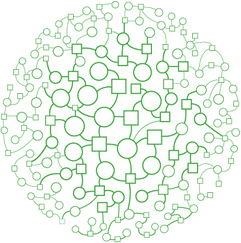
\includegraphics[height=3em]{filmat}
  \scalebox{0.5}{\sieve{14}{2}}
}

\newcommand{\muchstuffplaceholder}{
  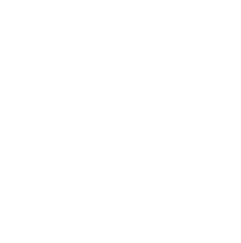
\includegraphics[height=3em]{filmat-placeholder}
  \scalebox{0.5}{\fakesieve{14}{2}}
}

\newcommand{\fewstuff}{
  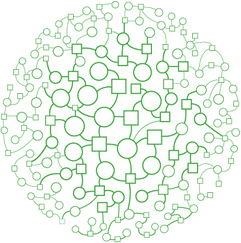
\includegraphics[height=3em]{filmat}
  \scalebox{0.5}{\sieve{7}{2}}
}

\newcommand{\threeblobs}{
  \colorbox{mypurple}{\ \ }\quad
  \colorbox{mypurple}{\ \ }\quad
  \colorbox{mypurple}{\ \ }
}

%\setbeamertemplate{headline}{\mynav{gray}{gray}{gray}}

{\usebackgroundtemplate{\begin{minipage}{\paperwidth}\vspace*{4.95cm}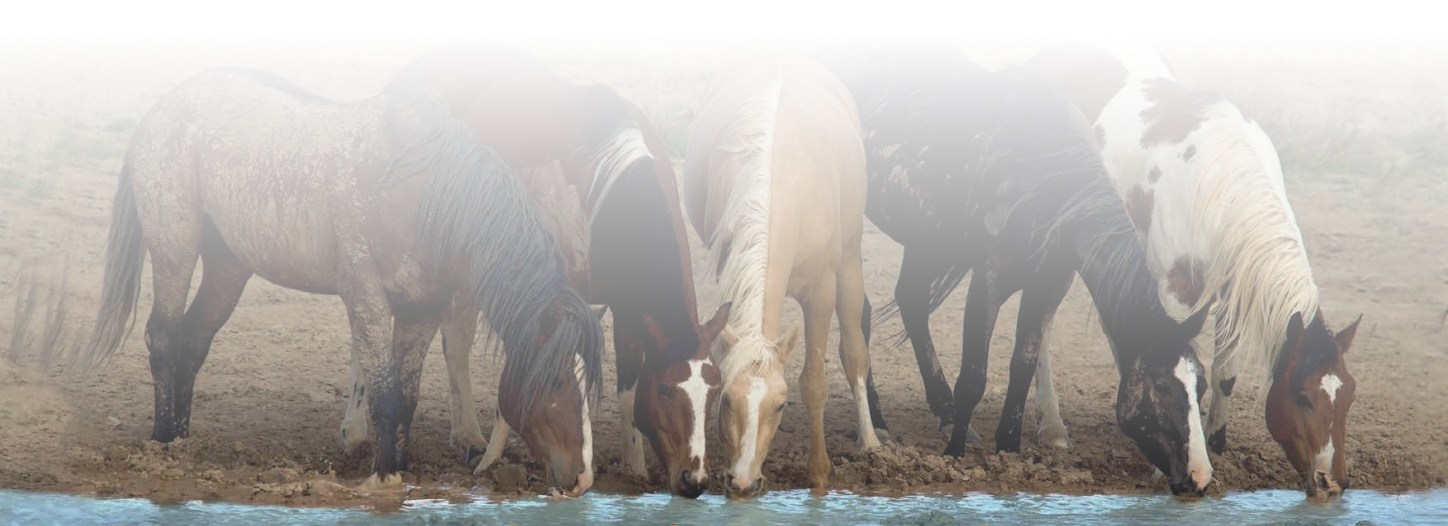
\includegraphics[width=\paperwidth]{topos-horses}\end{minipage}}
\begin{frame}[c]
  \centering

  \begin{tikzpicture}
    \def\R{8pt}
    \node (title) {\hil{\,Generalized spaces for constructive algebra\,}};
    \begin{pgfonlayer}{background}
      \draw[decorate, very thick, draw=mypurple]
        ($(title.south west) + (\R, 0)$) arc(270:180:\R) --
        ($(title.north west) + (0, -\R)$) arc(180:90:\R) --
        ($(title.north east) + (-\R, 0)$) arc(90:0:\R) --
        ($(title.south east) + (0, \R)$) arc(0:-90:\R) --
        cycle;
    \end{pgfonlayer}
  \end{tikzpicture}
  \bigskip

  \begin{columns}
    \small
    \begin{column}{0.35\textwidth}
      \centering
      \bignumber{1}
      
      \phantom{x}\hil{Locales}
      \medskip

      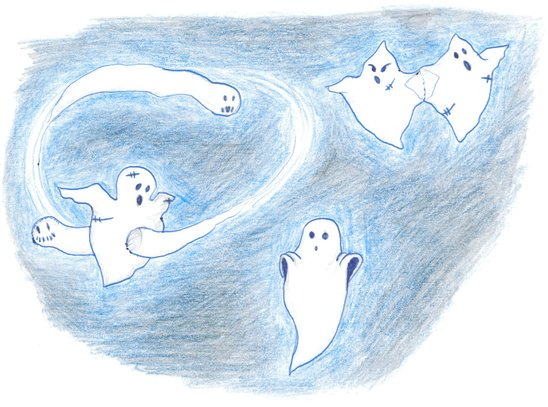
\includegraphics[height=4.5em]{phantoms.png}
    \end{column}
    \hspace*{0.5em}
    \begin{column}{0.28\textwidth}
      \centering
      \bignumber{2}

      \phantom{x}\hil{Sheaf models}
      \medskip

      \phantom{x}\!\!\begin{tikzpicture}
        \node (overview) {
          \scalebox{0.35}{\sieve{4}{3}}
        };
        \def\R{8pt}
        \begin{pgfonlayer}{background}
        \draw[decoration={bumps,segment length=8pt}, decorate, very thick, draw=mypurple]
          ($(overview.south west) + (\R, 0)$) arc(270:180:\R) --
          ($(overview.north west) + (0, -\R)$) arc(180:90:\R) --
          ($(overview.north east) + (-\R, 0)$) arc(90:0:\R) --
          ($(overview.south east) + (0, \R)$) arc(0:-90:\R) --
          cycle;
        \end{pgfonlayer}
      \end{tikzpicture}
    \end{column}
    \begin{column}{0.4\textwidth}
      \centering
      \bignumber{3}
      
      \hil{Constructive algebra}
      \medskip

      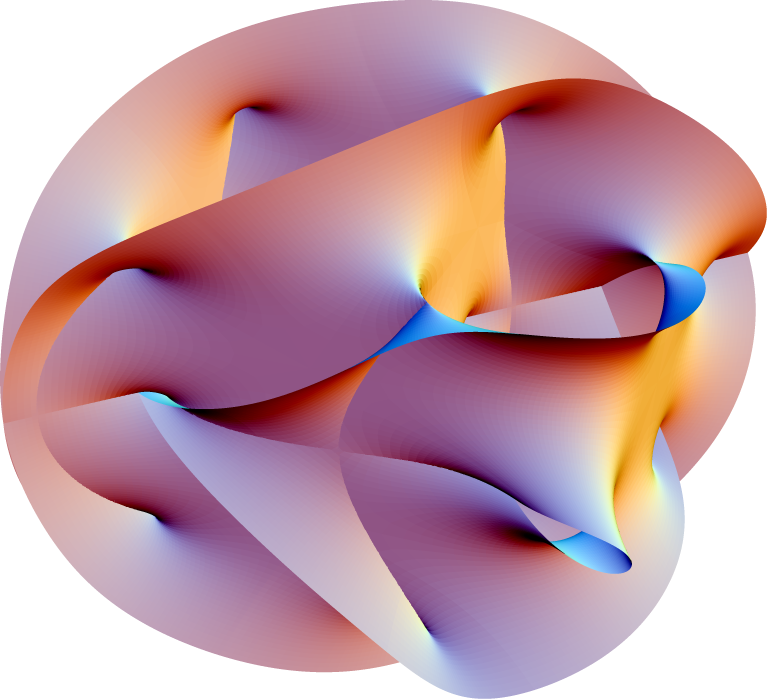
\includegraphics[height=4.5em]{calabi-yau}
    \end{column}
  \end{columns}
  \bigskip

  \scriptsize
  \textit{-- an invitation --}
  \bigskip

  Autumn school on Proof and Computation \\
  September 20th to 26th, 2019 \\
  Herrsching
  \bigskip

  Ingo Blechschmidt \\
  Università di Verona
  \par

\end{frame}}

% \begin{document}


\section{Locales}

\begin{frame}
  \centering\bigskip
  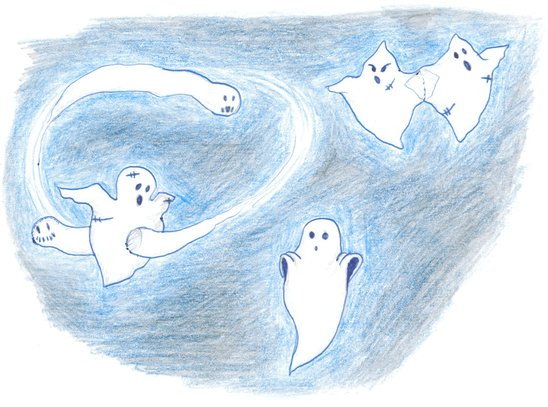
\includegraphics[height=9.5em]{phantoms}

  \large Lecture I:
  \hil{Locales}

  \normalsize

  \begin{hilblock}Locales are a kind of space in which \hil{opens} instead of
  \hil{points} are fundamental.\end{hilblock}

  \jnote{1}{
    These ``probability clouds'', replacing the reassuring material particles of
    before, remind me strangely of the elusive ``open neighborhoods'' that populate
    the topoi, like evanescent phantoms, to surround the imaginary ``points''.

    \hfill -- Alexander Grothendieck

    \bigskip
    \bigskip

    References include:
    \begin{enumerate}
      \item Peter Johnstone.
      \fixedhref{http://pointlesstopology.com/the-point-of-pointless-topology.pdf}{The point of pointless topology}, 1983.
      \item Peter Johnstone.
      \fixedhref{http://www.heldermann.de/R&E/RAE18/ctw06.pdf}{The art of
      pointless thinking: a student's guide to the category of locales}, 1990.
    \end{enumerate}

    Our metatheory is a constructive (no law of excluded middle, no choice
    principles of any kind) but impredicative (free use of the powerset axiom)
    flavor of English. The contents of this course could be formalized in the
    internal language of toposes or in~\textsc{izf}. The main ideas of this
    course are far more robust than this particular presentation, in
    particular, they can also be made sense of in a predicative setting (such
    as~\textsc{czf} or the internal language of arithmetic universes).
  }
\end{frame}

\begin{frame}{Locales in context}
  \justifying
  \textbf{Definition.} A \hil{topological space}~$X$ consists of a \hil{set of
  points} together with a set~$\O(X)$ of point sets which are deemed
  \hil{open} such that unions and finite intersections of open sets are open.
  \bigskip

  \centering\small
  \begin{tikzpicture}[sibling distance=8em, level distance=2.5em,
    every node/.style = {shape=rectangle, rounded corners,
      draw, align=center}, semithick, draw=mypurple]
    \node {euclidean spaces} [grow=up]
      child { node {metric spaces}
        child[dashed] { node [solid] {sober topological spaces}
          child[solid] { node {locales}
            child { node {toposes}
              child { node {$\infty$-toposes} } } }
          child[solid] { node {topological spaces} } } };
  \end{tikzpicture}
\end{frame}

\begin{frame}{Nontrivial spaces without points}
  The following locales don't have any points and are nontrivial:
  \begin{enumerate}
    \item the locale of surjections $\NN \twoheadrightarrow \RR$
    \item $\QQ \cap (\RR \setminus \QQ)$
    \item the pairwise intersections in the Banach--Tarski paradox
    \item Alex Simpson's locale of random binary sequences
  \end{enumerate}

  \begin{hilblock}
    Relinquishing points increases flexibility.
  \end{hilblock}

  \centering
  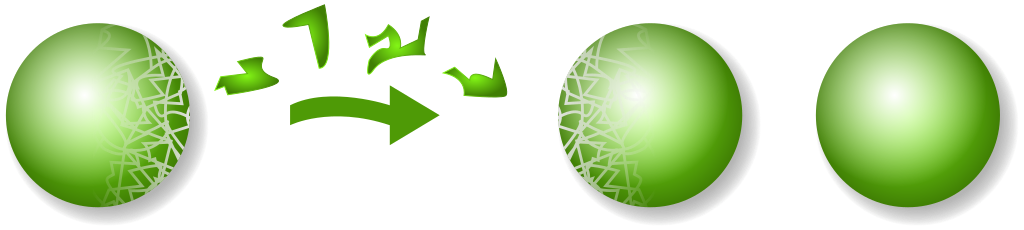
\includegraphics[height=5em]{banach-tarski}

  \jnote{1}{
    The locale of surjections $\NN \twoheadrightarrow \RR$ doesn't have any
    points, but it has lots of interesting opens, such as~$U_{n,x}$, the ``open of those
    surjections~$f$ such that~$f(n) = x$. If~$x$ is a fixed real number and~$n$
    ranges over the naturals, these opens cover the full locale.

    The Banach--Tarski paradox is the unintuitive statement that a
    three-dimensional solid ball of radius~$r$ can be partitioned into six
    disjoint subsets in such a way that rearranging those subsets yields two
    solid balls of radius~$r$ each. These subsets are not measurable and
    require the axiom of choice for their construction.

    The Banach--Tarski paradox can be resolved by adopting the axiom of
    determinacy instead of the axiom of choice, which entails that all subsets
    of~$\RR^3$ are measurable, or by passing from the topological space~$\RR^3$
    to its localic cousin. The localic counterparts of the six pieces will
    still not have any points in common, but their locale-theoretic pairwise
    intersection will not be trivial.

    Tom Leinster
    \fixedhref{https://golem.ph.utexas.edu/category/2011/12/on_the_law_of_large_numbers_su.html}{published
    an accessible exposition} of the locale of random sequences at the n-category café.
  }
\end{frame}

\begin{frame}{Issues of constructivity}
  \begin{enumerate}\justifying
    \item The unit interval~$[0,1]$ is \hil{compact}.
    \bigskip

    \item \hil{The fundamental theorem of Galois theory:}
    Let~$L | k$ be a Galois extension. Then there is a bijection between
    \[ \small\begin{array}{@{}rcl@{}}
      \begin{minipage}{0.25\textwidth}\centering the intermediate extensions~$L|E|k$\end{minipage}
      &\text{and}&
      \begin{minipage}{0.33\textwidth}\centering the closed subgroups
      of~$\mathrm{Aut}_k(L)$.\end{minipage} \\
      \\
      E &\longmapsto& \{ \sigma \in \mathrm{Aut}_k(L) \,|\, \sigma|_E = \operatorname{id} \} \\
      L^H &\longmapsfrom& H
    \end{array} \]
    \medskip

    \item \hil{Gelfand duality:} The categories of
    \[ \small\begin{array}{@{}rcl@{}}
      \begin{minipage}{0.38\textwidth}\centering compact Hausdorff spaces\end{minipage}
      &\text{and}&
      \left(\begin{minipage}{0.33\textwidth}\centering commutative $C^\star$-algebras with unit\end{minipage}\right)^{\mathrm{op}} \\[1.1em]
      X &\longmapsto& \{ f : X \to \CC \,|\, \text{$f$ continuous} \}
    \end{array} \]
    are equivalent.
  \end{enumerate}

  \jnote{1}{
    By \emph{compact}, we mean any open covering has a (Kuratowski-)finite
    subcovering. The topological space~$[0,1]$ fails to be compact in some
    flavors of constructive mathematics, but the localic unit interval is
    always compact.

    In verifying the fundamental theorem of Galois theory, at some point one
    has to extend a given~$k$-homomorphism~$E \to L$ which is defined on some
    finite intermediate extension~$E$ to~$L$. One-step extensions to larger
    intermediate extensions are no problem, but extending to all of~$L$
    requires some form of choice. By passing from the topological Galois group
    to its localic group, this issue vanishes. References include the papers
    \fixedhref{https://core.ac.uk/download/pdf/82660137.pdf}{Galois theory in a topos} and
    \fixedhref{http://www.numdam.org/article/CTGDC_1981__22_1_61_0.pdf}{Localic groups} by Gavin Wraith.
    Olivia Caramello's paper
    \fixedhref{https://arxiv.org/abs/1301.0300}{Topological galois theory} is
    also relevant.

    A similar issue arises with Gelfand duality. A fully constructive treatment
    is possible by passing from compact Hausdorff (topological) spaces to
    completely regular locales. This treatment unlocks the Bohr topos approach
    to quantum mechanics.
  }
\end{frame}

\begin{frame}{Localic basics}
  \justifying
  \textbf{Definition.} A \hil{topological space}~$X$ consists of a \hil{set of
  points} together with a set~$\O(X)$ of point sets which are deemed
  \hil{open} such that unions and finite intersections of open sets are open.

  \textbf{Observation.} The partial order~$\O(X)$ of open sets has
  \[ \small\begin{array}{@{}ccc@{}}
    \text{arbitrary joins}
    &\text{and}&
    \text{finite meets}, \\
    \bigvee && \wedge
  \end{array} \]
  and finite meets distribute over arbitrary joins:
  \[ U \wedge \bigvee_i V_i = \bigvee_i (U \wedge V_i). \]
  \vspace*{-1.2em}
  \pause

  \textbf{Definition.} A \hil{frame} is a partial order with arbitrary joins
  and finite meets such that the distributive law holds.

  \textbf{Definition.} A \hil{locale}~$X$ is given by a \hil{frame~$\O(X)$ of opens}.

  \jnote{2}{
    \textbf{Example.} Any topological space~$Y$ induces a locale~$L(Y)$ by
    setting~$\O(L(Y)) \defeq \O(Y)$.

    \textbf{Example.} The \emph{one-point locale}~$\pt$ is the locale induced
    by the one-point topological space~$\{\heartsuit\}$. Its frame of opens is
    the powerset of~$\{\heartsuit\}$, also known as the set~$\Omega$ of truth
    values. Its least element is~$\bot = \emptyset$ and its largest element
    is~$\top = \{\heartsuit\}$.

    \textbf{Definition.} A \emph{frame homomorphism}~$L \to L'$ is a monotone
    map~$L \to L'$ which preserves arbitrary joins and finite meets.

    \textbf{Example.} A continuous map~$f : Y \to Y'$ induces a frame
    homomorphism~$\O(Y') \to \O(Y)$ by mapping~$U \mapsto f^{-1}[U]$.

    \textbf{Definition.} A \emph{locale morphism}~$X \to X'$ is given by a
    frame homomorphism~$\O(X') \to \O(X)$.

    \textbf{Example.} A continuous map~$Y \to Y'$ induces a locale
    morphism~$L(Y) \to L(Y')$ in the same direction.

    \textbf{Definition.} A \emph{point} of a locale~$X$ is a locale
    morphism~$\pt \to X$, or equivalently a completely prime filter of~$\O(X)$.
    (A frame morphism~$\alpha : \O(X) \to \Omega$ gives rise to the completely prime
    filter~$F \defeq \{ u \in \O(X) \,|\, \alpha(u) = \top \}$.)
  }

  \jnote{3}{
    The set of points of a locale can be made into a topological space, giving
    rise to a functor~$\pt : \Loc \to \Top$. This functor is right adjoint
    to~$L$. A locale~$X$ is \emph{spatial} iff the canonical
    morphism~$L(\pt(X)) \to X$ is an isomorphism, and a topological space~$Y$
    is \emph{sober} iff the canonical morphism~$Y \to \pt(L(Y))$ is a
    homeomorphism.
  }
\end{frame}


% \begin{document}

\section{Sheaf models}

\begin{frame}
  \centering\bigskip
  \begin{tikzpicture}
    \node (overview) {
      \scalebox{1.00}{\sieve{4}{3}}
    };
    \def\R{8pt}
    \begin{pgfonlayer}{background}
    \draw[decoration={bumps,segment length=8pt}, decorate, very thick, draw=mypurple]
      ($(overview.south west) + (\R, 0)$) arc(270:180:\R) --
      ($(overview.north west) + (0, -\R)$) arc(180:90:\R) --
      ($(overview.north east) + (-\R, 0)$) arc(90:0:\R) --
      ($(overview.south east) + (0, \R)$) arc(0:-90:\R) --
      cycle;
    \end{pgfonlayer}
  \end{tikzpicture}

  \large Lecture II:
  \hil{Sheaf models}

  \normalsize

  \begin{hilblock}Sheaves allow us to explore mathematical objects from
  custom-tailored mathematical universes.\phantom{p}\end{hilblock}
\end{frame}

\begin{frame}{Frames presented by theories}
  \justifying
  \textbf{Definition.} A \hil{geometric theory} consists of
  \begin{enumerate}
    \small
    \item a set of sorts: $X$, $Y$, $Z$, \ldots
    \item a set of function symbols: $f : X \times Y \to Z$, \ldots
    \item a set of relation symbols: $R \hookrightarrow X \times Y \times Z$, \ldots
    \item a set of axioms: $\varphi \vdash_{x:X, y:Y} \psi$, \ldots
  \end{enumerate}

  \only<1->{
    \textbf{Examples.}
    The theory of rings,
    of surjections~\mbox{$\NN \twoheadrightarrow \RR$},
    of Dedekind cuts,
    of prime ideals of a given ring, \ldots
  }

  \textbf{Definition.} A \hil{set-based model}~$M$ of a theory~$\TT$ consists of
  \begin{enumerate}
    \small
    \item a set~$\brak{X}$ for each sort~$X$,
    \item a function~$\brak{f} : \brak{X_1} \times \cdots \times \brak{X_n} \to
    \brak{Y}$ \\
    for each function symbol~$f : X_1 \times \cdots \times X_n \to Y$, and
    \item a relation~$\brak{R} \subseteq \brak{X_1} \times \cdots \times
    \brak{X_n}$ \\
    for each relation symbol~$R \hookrightarrow X_1 \times \cdots \times X_n$
  \end{enumerate}
  such that~$M$ validates the axioms of~$\TT$.

  \jnote{1}{
    The formulas appearing to the left and the right of the turnstile in axioms
    of a geometric theory have to be \emph{geometric formula}. A formula is
    \emph{geometric} iff it is built using only~${=}\ {\top}\ {\wedge}\
    {\bot}\ {\vee}\ {\bigvee}\ {\exists}$ (but no ${\Rightarrow}\
    {\forall}$). Universal quantification and implication can to some extent be
    emulated by using free variables or the turnstile; but this allows
    universal quantification and implication only to be used once, on top
    level, not in nested subformulas.

    A geometric theory is called \emph{propositional} iff its set of
    sorts is empty. Hence the only ingredients of a propositional geometric
    theory are a set of nullary relation symbols (atomic propositions) and a
    set of axioms.
  }

  \jnote{2}{
    \textbf{Example.} The theory of rings has:
    \begin{enumerate}
      \item one sort: $R$
      \item five constant symbols: $0$ and $1$ (nullary), $-$ (unary), $+$ and
      $\cdot$ (binary)
      \item no relation symbols
      \item the usual axioms, such as $\top \vdash_{x:R,y:R} x + y = y + x$
    \end{enumerate}

    \textbf{Example.} The theory of surjections~$\NN \twoheadrightarrow \RR$ has:
    \begin{enumerate}\justifying
      \item no sorts
      \item no function symbols
      \item several nullary relation symbols, one for each pair~$\langle n,x
      \rangle \in \NN \times \RR$, written~``$\varphi_{nx}$''
      \item axioms: the axiom~$\top \vdash \bigvee_{x \in \RR} \varphi_{nx}$
      for each~$n \in \NN$; the axiom~$\varphi_{nx} \wedge \varphi_{ny} \vdash
      \bigvee\{ \top \,|\, x = y \}$ for each~$n \in \NN$, $x,y \in \RR$ (the
      disjunction appearing in that axiom is over a subsingleton of formulas);
      the axiom~$\top \vdash \bigvee_{n \in \NN} \varphi_{nx}$ for each~$x \in
      \RR$
    \end{enumerate}
  }

  \jnote{3}{
    Associated to any propositional geometric theory~$\TT$ is its
    \emph{Lindenbaum algebra}. This is the set of formulas over the signature
    of the theory modulo provable equivalence. Endowed with the partial order
    given by
    \[ [\varphi] \leq [\psi] \quad\vcentcolon\Longleftrightarrow\quad
      \text{$\TT$ proves $\varphi \vdash \psi$}, \]
    the Lindenbaum algebra becomes a frame.

    The Lindenbaum algebra of~$\TT$ is the free frame generated by the
    atomic propositions of~$\TT$ modulo the axioms of~$\TT$. The associated
    locale~$L(\TT)$ is the \emph{classifying locale of~$\TT$}. Its points are
    in canonical bijection with the set-based models of~$\TT$.

    \textbf{Definition.} The \emph{localic real line} is the classifying locale
    of the theory of Dedekind cuts.
    The \emph{locale of surjections~$\NN \twoheadrightarrow \RR$} is the
    classifying locale of the theory of surjections~$\NN \twoheadrightarrow
    \RR$.
    The \emph{empty locale} is the classifying locale of the \emph{inconsistent
    theory} (which has no sorts, no function symbols, no relations symbols, and
    one axiom, namely~$\top \vdash \bot$).

    The points of the localic real line are in canonical bijection with
    the Dedekind cuts, hence with the elements of the set of (Dedekind) real
    numbers. The points of the locale of surjections~$\NN \twoheadrightarrow
    \RR$ are in canonical bijection with the surjections~$\NN
    \twoheadrightarrow \RR$. Assuming a classical metatheory, there are no such
    points, but the locale is still nontrivial.
  }

  \jnote{4}{
    Any locale is (isomorphic to) the classifying locale of some propositional
    geometric theory, namely the ``theory of its points''. The same locale can
    often be presented by widely different-looking theories, and the
    topos-theoretic version of this observation is the basis for Olivia
    Caramello's research program.

    \textbf{Exercise.} Which explicit theory is the two-point locale (the
    locale induced from the discrete topological space~$\{0,1\}$) the
    classifying locale of?
  }
\end{frame}

\begin{frame}{Sheaves}
  \justifying
  \textbf{Definition.} A \hil{presheaf}~$F$ on a locale~$X$ is given by
  \begin{enumerate}
    \item a set~$F(U)$ for each open~$U$ of~$X$ and
    \item a map~$(\cdot)|^U_V : F(U) \to F(V)$ for each opens~$V \leq U$
  \end{enumerate}
  such that $(\cdot)|^U_U = \operatorname{id}_{F(U)}$ for all~$U$ and
  $(\cdot)|^V_W \circ (\cdot)|^U_V = (\cdot)|^U_W$ for all~$W \leq V
  \leq U$.
  A \hil{compatible family} with respect to a covering~$U = \bigvee_i U_i$
  is a family~$(s_i)_i$ of sections~$s_i \in F(U_i)$ such that~$s_i|^{U_i}_{U_i
  \wedge U_j} = s_j|^{U_j}_{U_i \wedge U_j}$. $F$ is a \hil{sheaf} iff for any
  such family there is a unique section~$s \in F(U)$ such that~$s|^U_{U_i} =
  s_i$ for all~$i$.

  \textbf{Example.} The \hil{sheaf of continuous functions} on a locale~$X$ is
  given by~$\C(U) = \Hom(U,\RR)$.

  \textbf{Non-example.} The \hil{presheaf of constant
  functions},~$\C_{\text{c}}(U) = \text{``the set of constant functions~$U \to
  \RR$''}$, is usually not a sheaf.

  \jnote{1}{
    All definitions on this slide literally also make sense for topological
    spaces instead of locales, since only the notion of opens and their
    inclusion relation is used.

    The maps~$(\cdot)|^U_V$ are called \emph{restriction maps}. For the
    sheaf~$\C$ of continuous real-valued functions, they are given by actual
    restriction of functions to smaller domains, that is by
    \[ \C(U) \longrightarrow \C(V),\ s \longmapsto s|_V. \]

    \textbf{Exercise.} Find, in the case~$X = [0,1]$, a compatible family of
    sections of the presheaf~$\C_\text{c}$ which shows that this
    presheaf is not a sheaf.
  }
\end{frame}

\begin{frame}{Sheaf semantics}
  \justifying\small
  Let~$X$ be a locale. We recursively define what it means for a
  \hil{first-order formula over an open~$U$ of~$X$} to be forced:
  \[ \footnotesize\renewcommand{\arraystretch}{1.08}\begin{array}{@{}l@{\ \ }c@{\ \ }l@{}}
  U \models \top &\Ll& \text{true} \\
  U \models \bot &\Ll& \hcancel{\text{false}}{0pt}{3pt}{0pt}{-2pt}\ U = \bot \\
  U \models s =_F t &\Ll& \text{$s = t$ when evaluated as elements of~$F(U)$} \\
  U \models \varphi \wedge \psi &\Ll&
  \text{$U \models \varphi$ and $U \models \psi$} \\
  U \models \varphi \vee \psi &\Ll&
  \hcancel{\text{$U \models \varphi$ or $U \models
  \psi$}}{0pt}{3pt}{0pt}{-2pt}\ \text{there exists a covering $U = \bigvee_i U_i$} \\
  && \quad\quad\text{such that for all~$i$: $U_i \models \varphi$ or $U_i \models \psi$} \\
  U \models \varphi \Rightarrow \psi &\Ll&
  \text{for all~$V \leq U$: }
  \text{$V \models \varphi$ implies $V \models \psi$} \\
  U \models \forall s \? F\_ \varphi(s) &\Ll&
  \text{for all $V \leq U$ and sections~$s_0 \in F(V)$: $V \models \varphi(s_0)$} \\
  U \models \exists s \? F\_ \varphi(s) &\Ll&
  \hcancel{\text{there exists $s_0 \in F(U)$ such that $U \models \varphi(s_0)$}}{0pt}{3pt}{0pt}{-2pt} \\
  &&
  \text{there exists a covering $U = \bigvee_i U_i$ such that for all~$i$:} \\
  && \quad\quad \text{there exists~$s_0 \in F(U_i)$ such that $U_i \models \varphi(s_0)$}
  \end{array} \]
  \textbf{Theorem.} If~$U \models \varphi$ and if~$\varphi$ entails~$\psi$
  intuitionistically, then~$U \models \psi$.

  \jnote{1}{
    A \emph{formula over an open~$U$} of~$X$ is a first-order formula (made up
    using~${=}\ {\top}\ {\wedge}\ {\bot}\ {\vee}\ {\Rightarrow}\ {\forall}\
    {\exists}$) over the signature which has one sort for each sheaf~$F$, one
    constant symbol of sort~$F$ for each section~$s \in F(U)$, one function
    symbol~$f : F \to G$ for each morphism of sheaves, and so on.

    \textbf{Proposition.} The sheaf semantics is monotone and local in the
    following sense: If~$V \leq U$, then~$U \models \varphi$ implies~$V \models
    \varphi$. If~$U = \bigvee_i U_i$ and if~$U_i \models \varphi$ for all~$i$,
    then~$U \models \varphi$.

    \textbf{Exercise.} For any formula~$\varphi$ over any open~$U$ of any
    locale~$X$, there is a largest open~$V \leq U$ such that~$V \models
    \varphi$. (Hint: Set~$V \defeq \bigvee\{ W \leq U \,|\, W \models \varphi \}$
    and exploit the monotonicity and locality of the sheaf semantics.)

    \textbf{Exercise.} For any formula~$\varphi$ over any open~$U$ of any
    locale~$X$, $U \models \neg\neg\varphi$ iff there exists an open~$V \leq U$
    which is dense in~$U$ such that~$V \models \varphi$.
  }
\end{frame}

\begin{frame}{Internalizing parameter-dependence}
  \justifying
  \small
  Let~$X$ be a topological space. Let~$(f_x)_{x \in X}$ be a continuous family of continuous
  functions~$\RR \to \RR$ (that is, let a continuous function $X \times \RR \to \RR,\,(x,a) \mapsto
  f_x(a)$ be given). This family defines a sheaf morphism~$f : \C \to
  \C$ by~$f_U : \C(U) \to \C(U),\,s \mapsto (x \mapsto f_x(s(x)))$.
  \normalsize

  \begin{itemize}\justifying
    \item $X \models \text{``$\C$ is the set of Dedekind real numbers''}.$
    \item $X \models \text{``the function $f : \C \to \C$ is
    continuous''}$.\medskip
    \item Iff $f_x(-1) < 0$ for all $x \in X$, then $X \models f(-1) < 0$.
    \item Iff $f_x(+1) > 0$ for all $x \in X$, then $X \models f(+1) > 0$.
    \item Iff all $f_x$ are increasing, then $X \models \text{``$f$ is
    increasing''}$.\medskip
    \item Iff there is an open cover~$X = \bigcup_i U_i$ such
    that for each~$i$, there is a continuous function~$s : U_i \to \RR$
    with~$f_x(s(x)) = 0$ for all~$x \in U_i$, then $X \models \exists s
    \? \C\_ f(s) = 0$.
  \end{itemize}

  \jnote{1}{Hence:
  \begin{enumerate}\justifying
    \item The standard formulation of the intermediate value theorem fails
    in~$\Sh(X)$, because its external interpretation is that in continuous
    families of continuous functions, zeros can locally be picked continuously.
    That claim is false, as
    \fixedhref{https://rawgit.com/iblech/internal-methods/master/images/zeros-in-families.mp4}{this
    counterexample} demonstrates.

    As a corollary, we deduce that the standard formulation of the
    intermediate value theorem is not constructively provable.

    \item The \emph{approximate} intermediate value theorem (stating
    that for any~$\varepsilon > 0$, there is a number~$x$ such that~$|f(x)| <
    \varepsilon$)
    \fixedhref{https://mathoverflow.net/questions/253059/approximate-intermediate-value-theorem-in-pure-constructive-mathematics}{has
    a constructive proof} and therefore holds in~$\Sh(X)$. The
    external interpretation is that in continuous families of continuous
    functions, approximate zeros can locally be picked continuously.

    \item The \emph{monotone} intermediate value theorem, stating that a strictly
    increasing continuous function with opposite signs has a unique zero,
    admits a constructive proof and therefore holds in~$\Sh(X)$. The external
    interpretation is that in continuous families of strictly increasing
    continuous functions, zeros can globally be picked continuously. You are
    invited to prove this fact directly, without reference to the internal
    language. This exercise isn't particularly hard, but it's not trivial either.
  \end{enumerate}}
\end{frame}


% \begin{document}

\section{Applications in constructive algebra}

\begin{frame}
  \centering\bigskip
  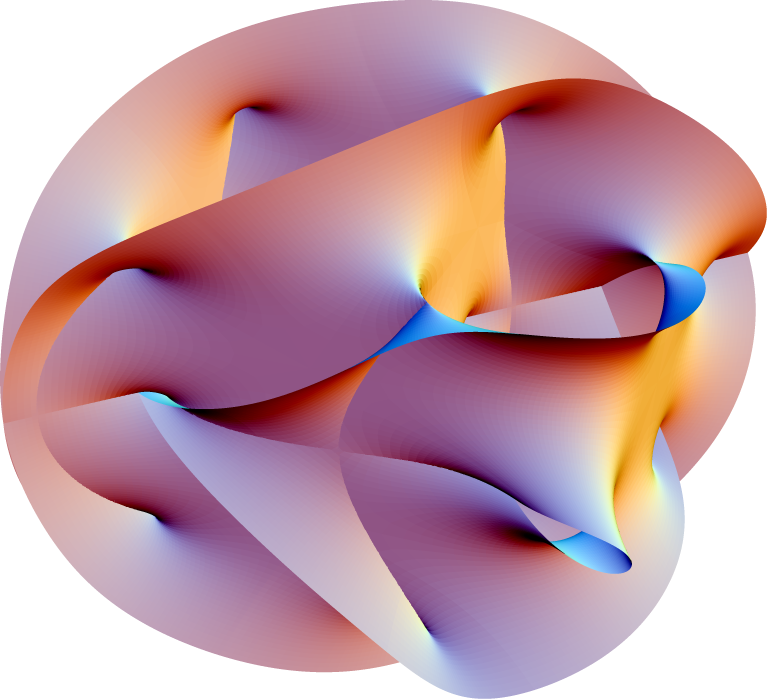
\includegraphics[height=8em]{calabi-yau}

  \large Lecture III:
  \hil{Applications in constructive algebra}

  \normalsize

  \begin{hilblock}Without loss of generality, any reduced ring is a field.\end{hilblock}
\end{frame}

\begin{frame}{A remarkable sheaf}
  \justifying
  Let~$A$ be a reduced ring ($x^n = 0 \Rightarrow x = 0$).
  Then there is a certain sheaf~$A^\sim$ of rings on a certain locale~$X$ such
  that \ldots

  {\centering $A^\sim$ is close to~$A$:\par}
  \vspace*{-1.4em}
  \begin{varblock}{\textwidth}{}
    \justifying
    There is a \hil{canonical bijection}~$A \to A^\sim(X)$.

    $A^\sim$ inherits any property of~$A$ which is
    \hil{localization-stable}.

    A geometric sequent holds for~$A^\sim$ iff$^\star$ it holds for \hil{all
    stalks}~$A_{\mathfrak{f}}$.
  \end{varblock}

  {\centering $A^\sim$ has better properties than~$A$:\par}
  \vspace*{-1.6em}
  \setbeamercolor{block body}{bg=red!30}
  \setbeamercolor{structure}{fg=purple}
  \begin{varblock}{\textwidth}{}
    $A^\sim$ is a \hil{field}: $\forall x\?A^\sim\_ (\neg(\exists y\?A^\sim\_
    xy = 1) \Rightarrow x = 0)$.

    $A^\sim$ has \hil{$\boldsymbol{\neg\neg}$-stable equality}:
    $\forall x,y\?A^\sim\_ \neg\neg(x = y) \Rightarrow x = y$.

    \mbox{$A^\sim$ is \hil{anonymously Noetherian}.}\\[-1.2em]
  \end{varblock}

  {\centering This observation can be exploited to give \\ short, conceptual and
  constructive proofs.\par}
\end{frame}

% XXX In note slides, explain "iff*".

\begin{frame}{Examples}
  \vspace*{-1.2em}
  \begin{columns}[t]
    \begin{column}[t]{0.58\textwidth}
      \centering

      \begin{varblock}{\textwidth}{Injective matrices}
        \justifying
        Let~$M$ be an injective matrix with more columns than rows over a ring~$A$.
        Then~$1 = 0$ in~$A$.
      \end{varblock}

      \justifying
      \textbf{Proof.} \bad{Assume not.} Then there is a \bad{maximal
      prime filter} $\fff \subseteq A$. The matrix is injective over the \bad{field}~$A_\fff$;
      contradiction to basic linear algebra.\medskip

      \textbf{Proof.} $M$ is also injective as a matrix over~$A^\sim$.
      This is a contradiction by basic linear
      algebra. Thus~$X \models \bot$. This amounts to~$1 = 0$ in~$A$.
    \end{column}

    \begin{column}[t]{0.46\textwidth}
      \centering

      \begin{varblock}{\textwidth}{Generic freeness\phantom{p}}
        \justifying
        Let~$M$ be a finitely generated~$A$-module.
        If~$f = 0$ is the only element of~$A$ such that~$M[f^{-1}]$ is a
        free~$A[f^{-1}]$-module, then~$1 = 0$ in~$A$.
      \end{varblock}

      \justifying
      \textbf{Proof.} See \href{https://stacks.math.columbia.edu/tag/051Q}{[Stacks Project]}.
      \medskip

      \textbf{Proof.} The claim amounts to \mbox{$X \models
      \text{``$M^\sim$}$}$\text{ is \hil{not not} free''}$. This statement
      follows from basic linear algebra over the field~$A^\sim$.
    \end{column}
  \end{columns}
\end{frame}

% XXX in note slides, explain which space X to take

\begin{frame}[plain]
  \centering
  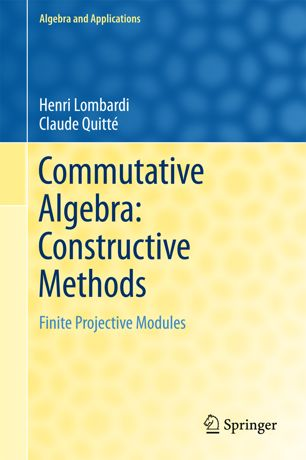
\includegraphics[height=\textheight]{lombardi-quitte}

  \jnote{1}{
    The book is \fixedhref{https://arxiv.org/abs/1605.04832}{available on the
    arXiv} and warmly recommended, as are all slides by Thierry Coquand on
    constructive algebra.
  }
\end{frame}
\addtocounter{framenumber}{-1}

\end{document}


% Grothendieck quote for the title picture:
%
% Ces “nuages probabilistes”, remplaçant les rassurantes particules matérielles
% d’antan, me rappellent étrangement les élusifs “voisinages ouverts” qui
% peuplent les topos, tels des fantômes évanescents, pour entourer des “points”
% imaginaires, ...
%
% Diese "Wahrscheinlichkeitswolken", welche die beruhigenden materiellen
% Partikel von früher ersetzen, erinnern mich irgendwie an die flüchtigen
% "offenen Umgebungen" der Topoi -- wie dahinschwindende Phantome, um
% die fiktiven "Punkte" zu umgeben, ...
%
% These “probability clouds”, replacing the reassuring material particles of
% before, remind me strangely of the elusive “open neighborhoods” that populate
% the topoi, like evanescent phantoms, to surround the imaginary “points”.
